\documentclass[letter,11pt,titlepage]{article}
\usepackage{lipsum}
\usepackage{graphicx}
\usepackage{amsmath}
\usepackage{listings}
\usepackage{float}
\usepackage{subcaption}
\begin{document}

\title{Who Said That?\\ \normalsize{Identifying Tweet Authors with Machine Learning}\\ \small{COSC522 (Machine Learning) Final Project Report}}
\author{Joseph Teague and Nigel Tan\\ \small{jteague6@vols.utk.edu and ntan1@vols.utk.edu}}
\maketitle

\begin{abstract}

    The ability to identify the author of a written work online is important for a number of reasons. While posts are typically tied to a username, individuals can have more than one account on many services and some individuals or organizations have a social media team to handle online posting for them. Author identification can, among other things, assist with tracking down users who are attempting to evadea ban or the author of a post that violates the policies of a celebrity or organization. In this work, we present an attempt to utilize machine learning to identify the individual author of a post. Using a number of machine learning techniques, we show results that have good sensitivity but poor specificity. We show through this work the difficulty of obtaining a reasonable classifier for this type of work without advanced techniques beyond the scope of a relatively short assignment.

\end{abstract}

\section{Introduction}

There is lots of publicly available work for sentiment analysis of Twitter posts (e.g., \cite{TSA1}, \cite{TSA2}, \cite{TSA3}). More work has been done to isolate interests \cite{TIA1} or location \cite{TLA1} of known Twitter users. However, none of this work focuses on identifying potentially unknown Twitter users. At first glance, this may not seem like a worthwhile endeavour. After all, every Twitter user has a username, which provides some level of reduction of anonyminity without necesarilly compromising a real world identity. However, we believe this work could prove beneficial for a number of reasons, primarily ban circumvention detection and ``team post'' author identification. In the former case, author identification could be used to potentially identify users who have attempted to circumvent a ban via the creation of a new account by comparing unknown posts to those from the known, banned account. In the latter case, an individual writer on a social media team could be identified to, for example, locate the origin of a particularly offensive post.

Machine learning is an obvious technique for attempting author identification. However, there are questions about how well it works (and what methods to use) and what features to select from raw text, given that anything like natural language processing is beyond our capabilities. To this end, we examined several supervised (e.g., kNN and SVM) and unsupervise (e.g. k-Means) methods for machine learning and experimented with the features extracted from the text.

The end result, explained in this document, is a complex examination methodology to address the pros and cons of various features and machine learning methods for author identification.

\section{Approach}

\subsection{The Dataset}

We obtained archives containing a number of Tweets from prolific celebrity Twitter users from Kaggle \cite{TweetSource}. While this archive contains a large number of users, we selected six who we thought would provide a diversity of writing style for the purposes of this examination. Those six are Donald Trump, Hillary Clinton, Richard Dawkins, Neil DeGrasse Tyson, Astronaut Scott Kelly, and Kim Kardashian. The Tweets provided are purely text and have no features extracted, so the dity of identifying features fell to us. The features we selected are:

\begin{itemize}
    \item Repeated punctuation (e.g., ``!!!!!'')
    \item Inclusion of images
    \item @s directed at other users or organizations
    \item Typing in all caps (e.g., ``NO COLLUSION'')
    \item Inclusion of links
    \item Quotations (e.g., "...")
    \item Use of hashtags (e.g. ``\#mancrushmonday'')
    \item Quotes
\end{itemize}

We also, as a comparison, run some tests with highly user-specific features extracted. These typically consist of things that one person is more likely to say than the others. For example, Donald Trump is more likely to say ``make America great again,'' while Scott Kelly is the only selected user who would discuss his time in space. These features target specific words and phrases and do not include any sort of natural language processing. The bulk of our tests do not include these highly-specific features, and the end goal is to develop a user-agnostic approach to author identification.

\subsection{Techniques Used}

Every technique used in class so far has been employed in this work. We use MPP cases 1, 2, and 3, k-Nearest-Neighbors, support vector machines (linear, poly, and sigmoid), and backpropagating neural networks were used for supervised learning methods. For unsupervised methods, k-Means, winner-take-all, and Kohonen maps were employed. We also employed decision trees, which were not used in class.

Each learning method was run multiple times (with a parameter sweep where appropriate) with m-fold cross validation to examin its effectiveness. In addition to total accuracy, we paid close attention to sensitivity and specificity. Computing performance was not measured - in this case, we are more interested in overall accuracy than anything else.

\section{Experiments}

All experiments used for this work were written in Python 3. Whereever possible, we canibalized code from our previous class assignments. The MPP case 1, 2, and 3 code came from  Project 1 \cite{Project1}. Code for k-Nearest-Neighbors, PCA, and FLD came from Project 2 \cite{Project2}. The backpropagating neural network code was adapted from Project 3 \cite{Project3}. Finally, Project 4 \cite{Project4} provided the framework for the unsupervised learning code (k-Means, winner-take-all, and Kohonen maps). Decision trees and SVM were implemented using SKLearn. Classifier fusion code was written from scratch for this project, as pre-existing code was written for a homework assignment and was found to be lacking for the purposes of this work.

The following series of experiments were designed to highlight several factors of classification methods. How the prior probability ratios affect classification accuracy. The impact of different common Minkowski distances. The performance changes introduced by classifier fusion. How effective different dimension reduction methods with regards to classification accuracy.

\section{Results}

\begin{figure}[H]
\begin{subfigure}[b]{0.5\linewidth}
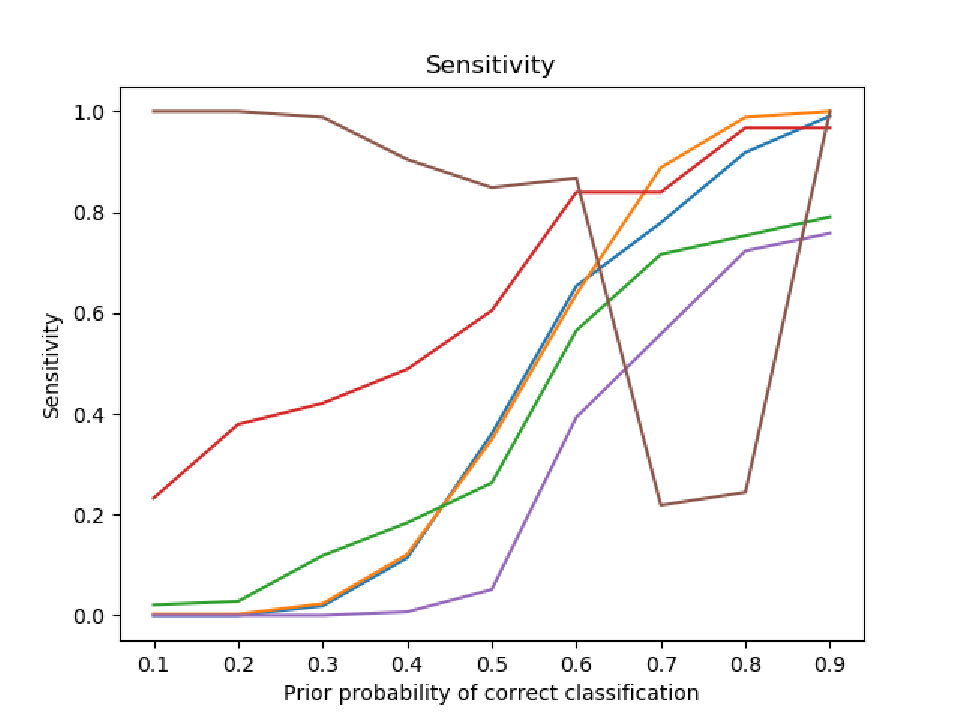
\includegraphics[width=7cm]{mpp_knn_fuse_sens.pdf}
\caption{Sensitivity of MPP and KNN}
\end{subfigure}
\begin{subfigure}[b]{0.5\linewidth}
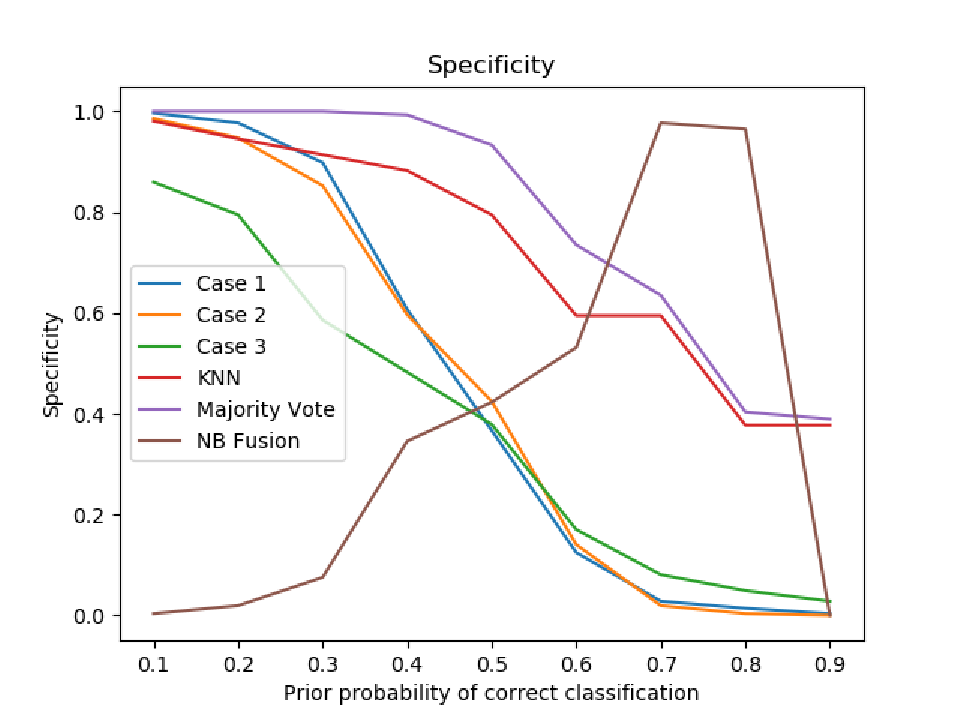
\includegraphics[width=7cm]{mpp_knn_fuse_spec.pdf}
\caption{Specificity of MPP and KNN}
\end{subfigure}
\caption{MPP and KNN performance both individual and fused with varying probability}
\end{figure}

\begin{figure}[H]
\begin{subfigure}[b]{0.5\linewidth}
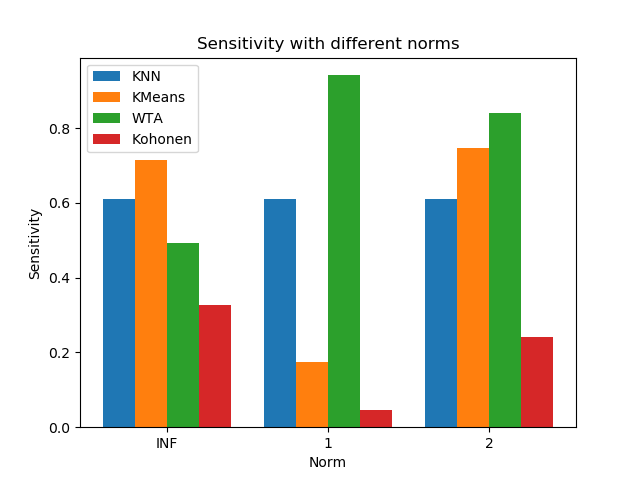
\includegraphics[width=7cm]{sens_with_norms.png}
\caption{Sensitivity of KNN, KMeans, Winner-take-all, and Kohonen Maps}
\end{subfigure}
\begin{subfigure}[b]{0.5\linewidth}
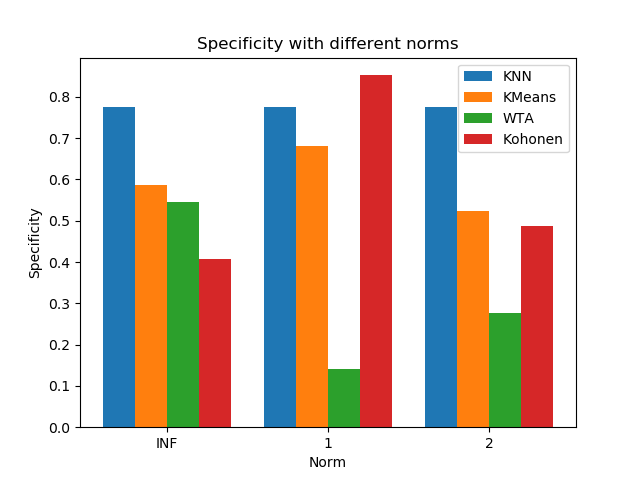
\includegraphics[width=7cm]{spec_with_norms.png}
\caption{Specificity of KNN, KMeans, Winner-take-all, and Kohonen Maps}
\end{subfigure}
\caption{Performance of KNN, KMeans, Winner-take-all, and Kohonen Maps with different Minkowski distances}
\end{figure}

\begin{figure}[H]
\centering
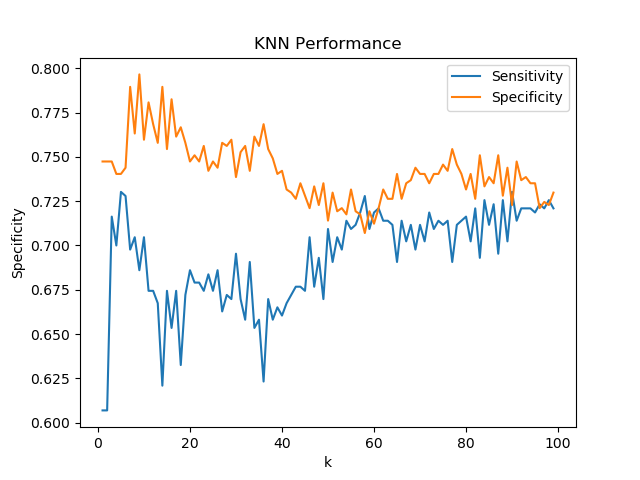
\includegraphics[width=\linewidth]{knn_sens_spec_plot.png}
\caption{kNN performance with varying k}
\end{figure}

\begin{figure}[H]
\centering
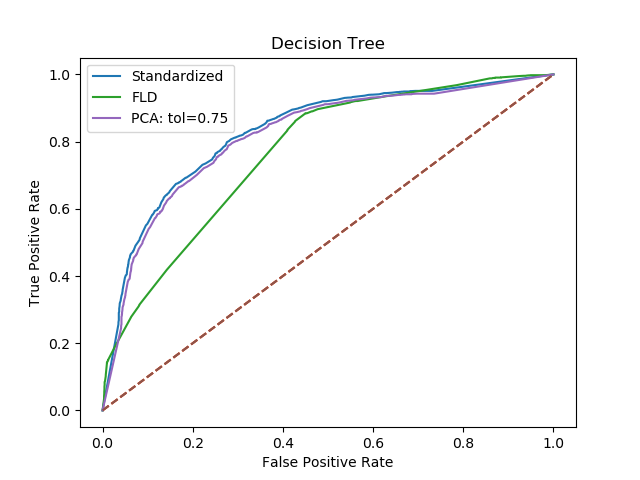
\includegraphics[width=\linewidth]{decision_tree.png}
\caption{Comparing Standardization vs FLD vs PCA for Decision Trees}
\end{figure}

\begin{figure}[H]
\centering
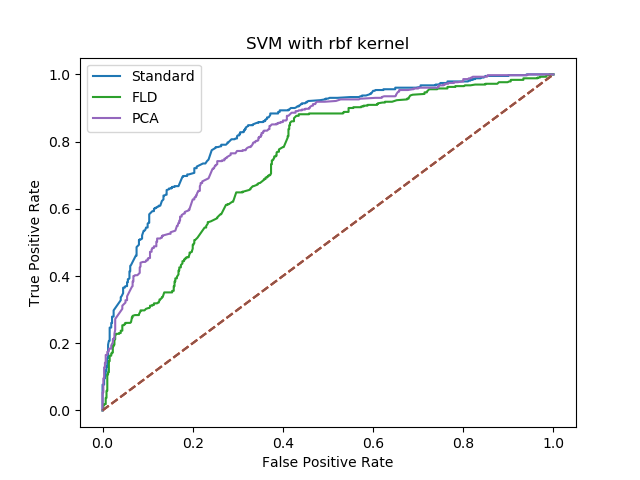
\includegraphics[width=\linewidth]{svm_dim_reduction.png}
\caption{Comparing Standardization vs FLD vs PCA (0.75 tolerance) for SVM using the rbf kernel}
\end{figure}

\begin{figure}[H]
\centering
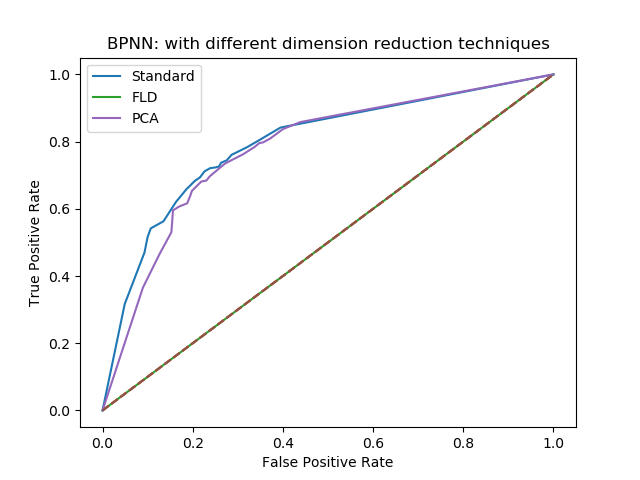
\includegraphics[width=\linewidth]{bpnn_dim_reduction.png}
\caption{Comparing Standardization vs FLD vs PCA (0.75 tolerance) for Back propagating neural network (1 hidden layer with 10 neurosn, 1000 epochs, online training, and e=0.1)}
\end{figure}

\begin{figure}[H]
\centering
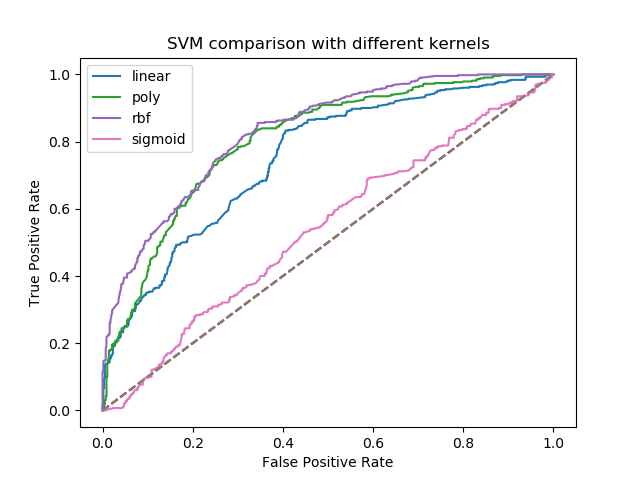
\includegraphics[width=\linewidth]{svm_comparison.png}
\caption{SVM with different kernels}
\end{figure}

\section{Discussion}

Using the features we selected, no learning model is ideal. While kNN and SVM+RBF provided decent results, accuracy that is only in the 70s as a best case is still not superb. As for the other models, the low-sensitivity high-specificity seen with the supervised techniques and the high-sensitivity low-specificity seen with the unsupervised techniques are not encouraging. After all, being able to tell that Donald Trump wrote something is not enough - you have to be able to tell if he DIDN'T write something, too. The failure of any one model to provide GOOD results highlights the complexity of this sort of work.

Varying the prior probability had somewhat expected effects. The sensitivity and specificity had near inverse relationships. All of the MPP cases had poor performance, barely crossing a coin flip in most cases. kNN on the other hand had significantly better performance. Classifier fusion between the various methods had limited and unpredictable benefits. In general fusing the different MPP classifiers with kNN resulted in better performance than MPP by itself but inferior compared to kNN. This highlights how the features selected do not form a nicely structure gaussian distribution. kNN had much better results but is much more computationally expensive. One nice factor about kNN is how easily it is to test different numbers of neighbors. Figure 3 clearly shows that with larger k values the performance improves.

Changing the distance metric for kNN, KMeans, Winner-take-all, and Kohonen Maps has little benefit compared to the standard 2 norm distance. kNN in particular was completely unaffected by the different metric choice. The further tests with decision trees, back propagating neural networks, and support vector machines highlight how FLD has little benefit while the data set is extremely lopsided with regards to features. Even with a 0.75 tolerance the standard and PCA results are nearly identical across the board.

SVM was interesting as the kernel choice had a significant affect on the performance based on how well it matched the data. One thing that was immediately apparent is how the supervised methods with MPP as the exception performed far better than the unsupervised methods.  

\section{Appendix}

\clearpage
\bibliography{sources}
\bibliographystyle{ieeetr}

\end{document}
